\section{Responsible AI}
\label{sec:appendix:ra}



In line with our expectations to build systems responsibly, we focus our efforts on the evaluation of added toxicity and bias. Both of these dimensions of responsible AI have drawn significant scientific attention in recent times (e.g., \citep{kiritchenko-et-al-2021,bender-et-al-2021,costajussa:nature:2019}). Moreover, the occurrence of these unintended errors or translation faults could adversely impact user experiences. Sustained attention devoted to such issues is, thus, vital to the safe deployment of our systems. 

Beyond these dimensions, we are also concerned with the concept of fairness. In contrast to the idea of robustness (as conceptualized in section \ref{subsec:robustnessspeakervariation}), where the focus is on whether our system performance is affected by the varying qualities of a speaker's voice, fairness in this section is more concerned about the \textit{content} of the translation outputs. Fair outputs do not preference or skew towards particular demographics and tend to treat different groups somewhat equitably. We document the results of these evaluations to better direct mitigation efforts.

\subsection{Definitions}
\label{sec:rai-def-back}
We begin by detailing how we define errors that arise from \textit{added toxicity} and \textit{gender bias}.

\paragraph{Toxicity.}  
In their taxonomy of critical machine translation errors, \citep{sharou-specia-2022-taxonomy} define ``deviation in toxicity'' as ``instances where the translation may incite hate, violence, profanity, or abuse against an individual or a group (a religion, race, gender, etc.) due to incorrect translations,'' which ``covers cases where toxicity is introduced into the translation when it is not in the source, deleted in the translation when it is in the source, mistranslated into different (toxic or not) words, or not translated at all (i.e., the toxicity remains in the source language or transliterated).'' Our definition of \textit{added toxicity} departs slightly from theirs in that it does not cover instances of untranslated toxic source content or of toxic source content deleted in the translation. To put it simplistically, added toxicity is the introduction of toxic elements not present in a source utterance.


\paragraph{Gender Bias.} Another error with which responsible AI is concerned lies in the propagation and amplification of gender bias. In machine translation, gender bias is observed when translations show errors in linguistic gender determination despite the fact that there are sufficient gender clues in the source content for a system to infer the correct gendered forms. To illustrate this phenomenon, sentence (1) below does not contain enough linguistic clues for a translation system to decide which gendered form should be used when translating into a language where the word for \textit{doctor} is gendered. Sentence (2), however, includes a gendered pronoun which most likely has the word \textit{doctor} as its antecedent.
\begin{enumerate}
\item I didn't feel well, so I made an appointment with my doctor.
\item My doctor is very attentive to \textbf{her} patients' needs.
\end{enumerate}
Gender bias is observed when the system produces the wrong gendered form when translating sentence (2) into a language that uses distinct gendered forms for the word \textit{doctor}. A single error in the translation of an utterance the like of sentence (1) would not be sufficient to conclude that gender bias exists in the model; doing so would take consistently observing one linguistic gender over another.
It has previously been hypothesized that one possible source of gender bias is gender representation imbalance in large training and evaluation data
sets, e.g. \citep{NEURIPS2022_09933f07,qian-etal-2022-perturbation}.








\subsection{Toxicity}
\label{apx:toxicity}

Warning: this section contains examples that may be offensive to some.



\subsubsection{Motivation}


\paragraph{Context} As mentioned above, added toxicity means introducing toxicity in the translation output not present in the input. This can be classified as a critical error; one that could lead users to distrust a translation system. As such, it is important to quantify how much toxicity our models add. We are also interested in combining added toxicity analysis with demographic bias analysis to determine whether added toxicity is generated more in certain demographic axes than in others.

\paragraph{Related work} While related research in speech toxicity detection is quite limited \citep{10.1007/978-3-030-60276-5_19,DBLP:conf/eusipco/YousefiE21}, toxicity detection for text-based approaches has been widely explored in different contexts. Many examples of these efforts can be found in large evaluations like JigSaw Series Kaggle Competitions\footnote{https://www.kaggle.com/c/jigsaw-toxic-comment-classification-challenge} or WMT Critical Error detection \citep{specia-etal-2021-findings}. Recently, in the context of \mt, there has been a substantial push to scale toxicity detection by using a word-list-based detection method for models such as NLLB \citep{nllb2022}, which further spurred research into analyzing toxicity at scale \citep{costajussa2023toxicity} and mitigation strategies \citep{gilabert2023resetox}.  %
Using a dataset that covers different demographic axes can allow for further analysis of which demographic axes are most sensitive to toxicity \citep{costajussa2023toxicity}. So far, datasets that cover a wide range of demographic axes mostly focus on text and more attention needs to be directed at speech (an example of a text data is \holisticbias \citep{smith-etal-2022-im}).



\paragraph{Proposed methodology} 

Inspired by \asrbleu, this work proposes using \asretox as a new metric to detect added toxicity in speech and evaluate added toxicity for \mfourt's \sst capability. Essentially, this metric follows a cascaded framework by first deploying a standard ASR module (i.e., the same that it is used for \asrbleu as defined in Table \ref{tbl:eval:metrics}), then the toxicity detection module, ETOX \citep{costajussa2023toxicity}, which uses the Toxicity-200 word lists. %
For \st, the translated output can be directly evaluated with ETOX. In both cases (\sst and \st), we measure added toxicity at the utterance/sentence level. We first compute toxicity detection for each input in the evaluation dataset and the corresponding output. Then we compare them and count a case as containing added toxicity only when the output value exceeds the one displayed by the input. %





\subsubsection{Experimental Framework}
\label{sec:expframetoxicity}

\paragraph{Language directions and modalities} Similarly to the previous human evaluation framework in Section \ref{subsec:appendix:humanmetrics}, we evaluated \sst and \st on \fleurs. Distinctive from human evaluation, we extended toxicity evaluation to cover all languages for which we provide translations for as summarized in Table \ref{tab:all_languages}. Igbo, Burmese, Nepali, and Assamese have issues related to segmentation and consistencies in the toxicity word lists.%
With these problems, these languages tend to over-detect toxicity and we consider them to be outliers. Therefore, we excluded them from the analysis and results.


\paragraph{Datasets} We used two datasets to analyze added toxicity. One, we used \fleurs to better align with our human evaluation effort and other evaluative components of this work. %
In addition, %
we used the English-only \holisticbias framework \citep{smith-etal-2022-im}, which has been shown to trigger true added toxicity in previous studies \citep{costajussa2023toxicity}. %
\holisticbias comprises 26 templates, encompassing more than 600 descriptors across 13 demographic axes, along with 30 nouns. The dataset consists of over 472K English sentences utilized in the context of two-person conversations. Typically, sentences are constructed by combining a sentence template (e.g., "I am a [NOUN PHRASE]."), a noun (e.g., parent), and a descriptor (e.g., disabled). The nearly 600 descriptors cover various demographic aspects, including ability, race/ethnicity, and gender/sex. The nouns may indicate a specific gender (e.g., woman, man) or avoid gender references (e.g., child, kid). Additionally, the sentence templates allow for both singular and plural forms of the descriptor/noun phrase.


In this work, we extend \holisticbias to speech by applying the default “en” transformer-tts model from fairseq S{\^{}}2
(\citep{wang-etal-2021-fairseq}). %
It first converts input texts into IPA phonemes, then passes them to a mel spectrogram generator transformer model
, and finally feeds the outputs to a HiFi-Gan vocoder to create the waveform. %




\paragraph{Models} As a baseline system for \st\ \xeng, we employ \whisperlarge~\citep{whisper}. As for \sst~\xeng, we apply the \cite{casanova2022yourtts} to generate synthesized speech from the output of \whisperlarge\ \st. For \st\ \engx, we employ the cascade system of \whisperlarge + \nllbmedium~\citep{nllb2022}.
Below, we report results for \mfourtlg.%

\paragraph{Evaluation} We use the Github implementation of ETOX\footnote{https://github.com/facebookresearch/stopes/tree/main/demo/toxicity-alti-hb/ETOX} For languages without spaces, we use the spm tokenization option in the tool.
For \asr, we use the same implementation framework used for \asrbleu as reported in Table \ref{tbl:eval:metrics}. %

\subsubsection{Results}

\paragraph{Automatic toxicity detection on \fleurs} We evaluated the output of \mfourtlg on the \fleurs dataset. 
\Cref{xxtoen-toxicity-s2t} presents results from \st and \sst for \xeng and \engx directions, where we show the number of sentences that contain added toxicity. When looking at the amount of added toxicity per sentence, less than 5\% of the cases contain more than 1 added toxicity token per sentence. Overall, \fleurs shows a relatively low prevalence of added toxicity of 0.15\%, averaging across languages, tasks, and translation directions. %


For \st  in \xeng  (Figure \ref{xxtoen-toxicity-s2t} (left)), added toxicity is 0.11\% averaged across languages, and 27 language pairs contain some added toxicity. For \sst (Figure \ref{xxtoen-toxicity-s2t} (right)), added toxicity is 0.12\% averaged across languages, and 35 language pairs contain added toxicity. 
  
For \st in \engx, (Figure \ref{xxtoen-toxicity-s2t} (left)), added toxicity is 0.21\% averaged across languages, and 32 language pairs contain added toxicity. For \sst (Figure \ref{xxtoen-toxicity-s2t} (right)), added toxicity is 0.16\% averaged across languages, and 16 language pairs contain added toxicity. The main difference across modalities is the reduced amount of added toxicity in \sst for the \engx translation direction. We comment on this difference alongside the results from the \holisticbias dataset later in this section.

By comparison, for \st in \xeng, \whisperlarge's added toxicity is 0.31\% averaged across languages and is prevalent in 58 languages. For overlapping languages in \whisperlarge and \mfourtlg, the latter shows an added toxicity reduction of 63\%. For \sst in \xeng , \whisperlarge + \yourtts's added toxicity lies at 0.27\% averaged across languages and is prevalent in 52 languages.%
Again, for overlapped languages in this cascaded \sst system and \mfourtlg, %
ours show a reduction of toxic tokens by 62\%. For \st in \engx, the \whisperlarge + \nllbmedium cascaded combination adds toxicity by 31\% averaged in languages and added toxicity is prevalent in 39 languages. For overlapping languages, \mfourtlg reduces this amount by 26\%. The filtering of imbalanced toxicity in the training data as reported in Section \ref{sec:modeling:x2t:data} may have contributed to this improvement.

\begin{figure}[h!]
    \centering
\noindent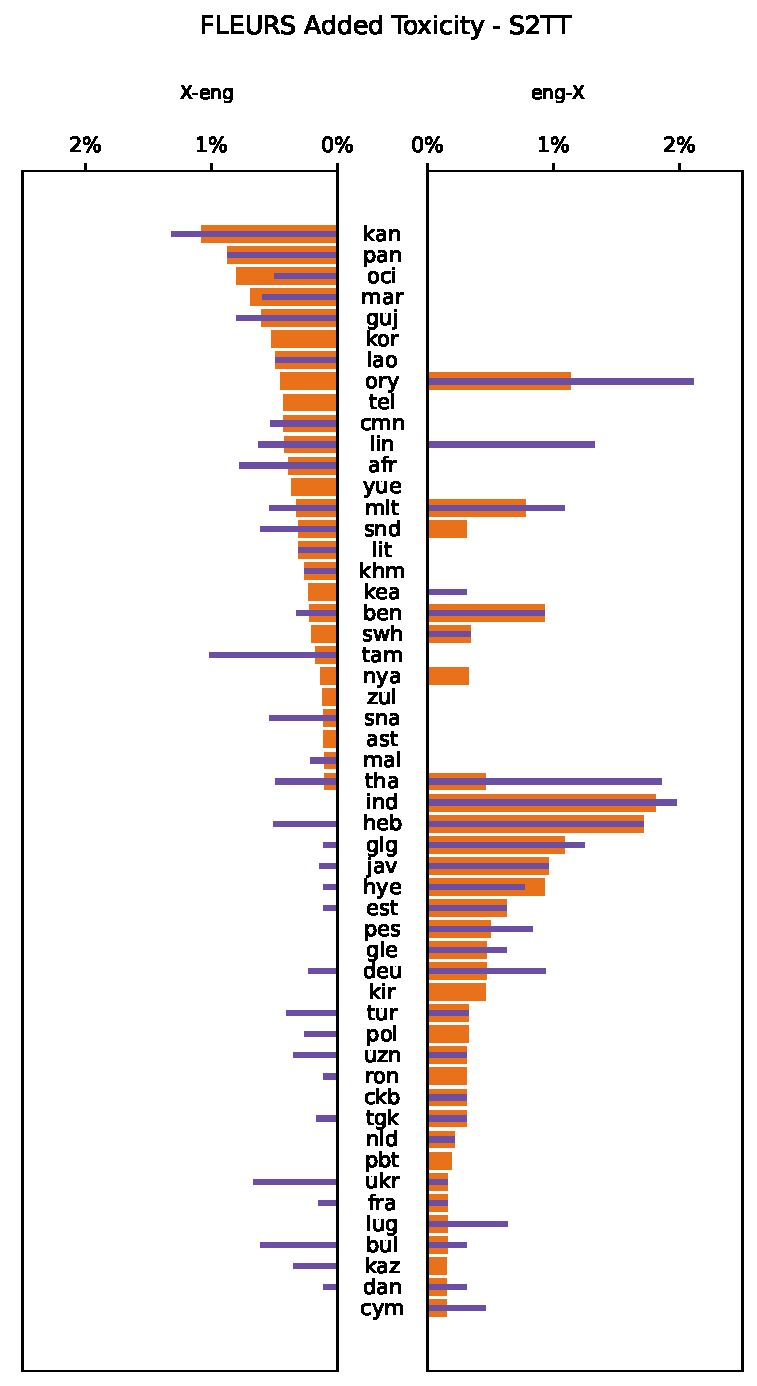
\includegraphics[width=.45\linewidth]{figures/rai/butterfly_fleurs_s2t_baseline.pdf}
\noindent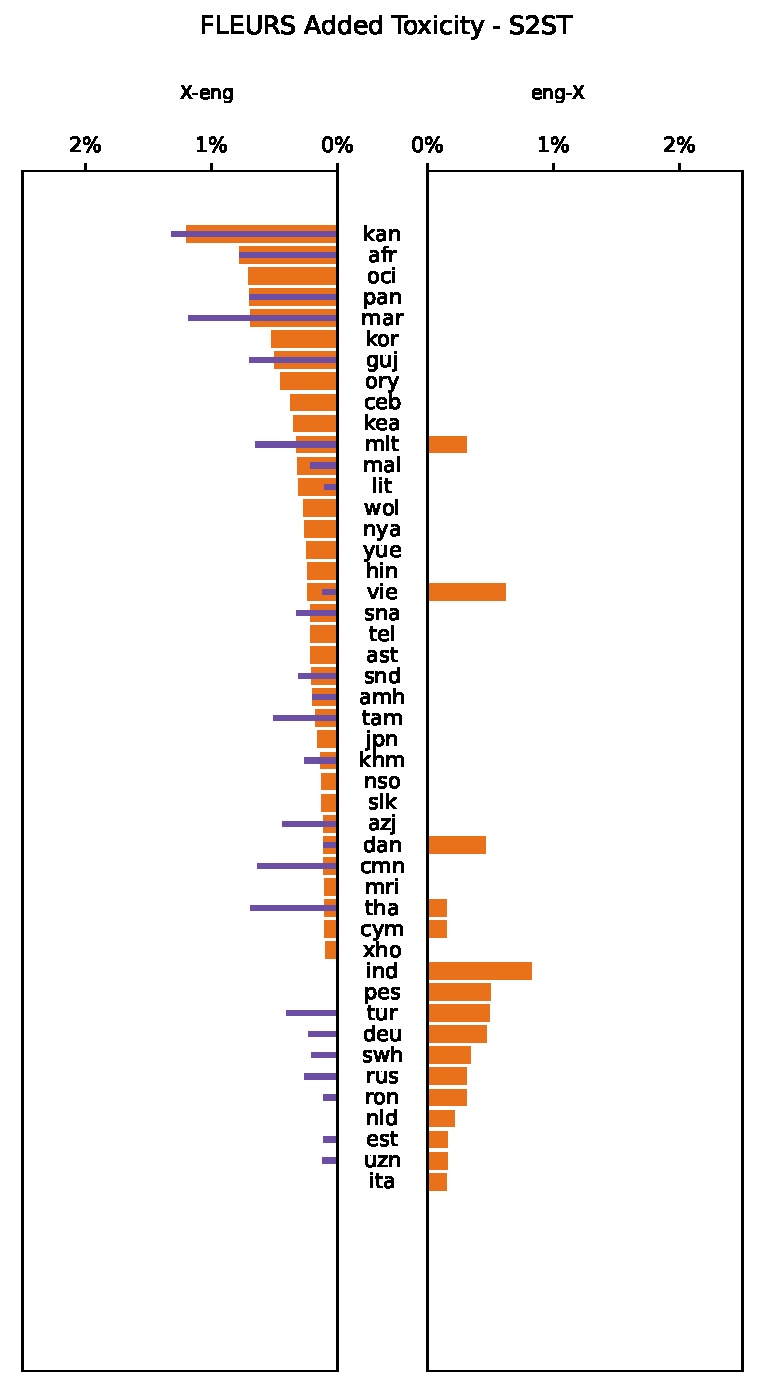
\includegraphics[width=.45\linewidth]{figures/rai/butterfly_fleurs_s2st_baseline.pdf}
    \caption{\label{xxtoen-toxicity-s2t} Added toxicity for \xeng and \engx for \st (left) and \sst (right) in \fleurs. The figure shows the number of outputs with added toxicity per language both for \mfourtlg (orange) and \whisperlarge and \whisperlarge + \yourtts systems when available (blue).}
\end{figure}







\begin{figure}[h!]
    \centering
\noindent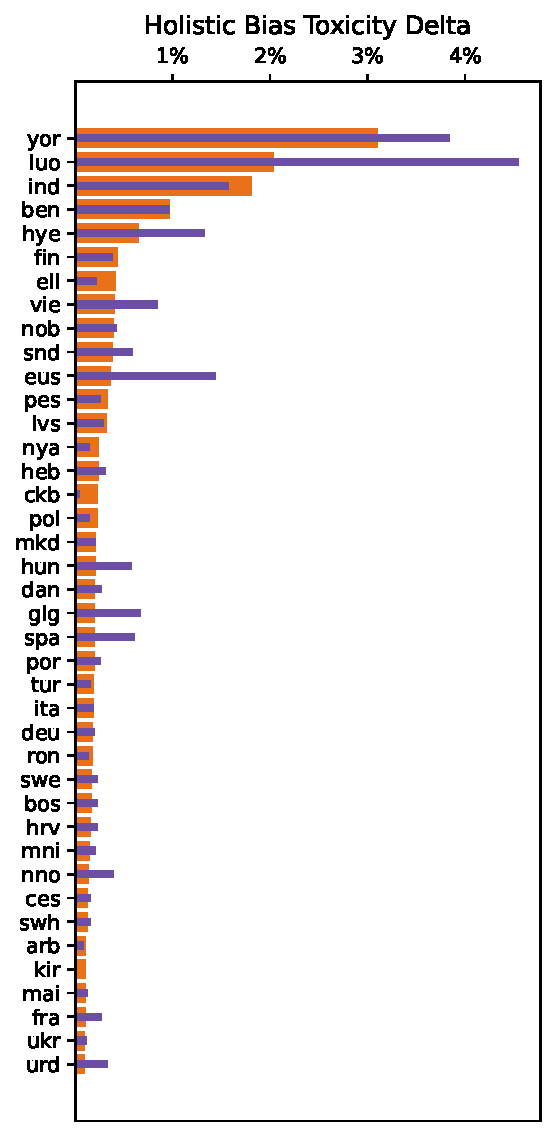
\includegraphics[width=.28\linewidth]{figures/rai/butterfly_hb_s2t_baseline.pdf}
\noindent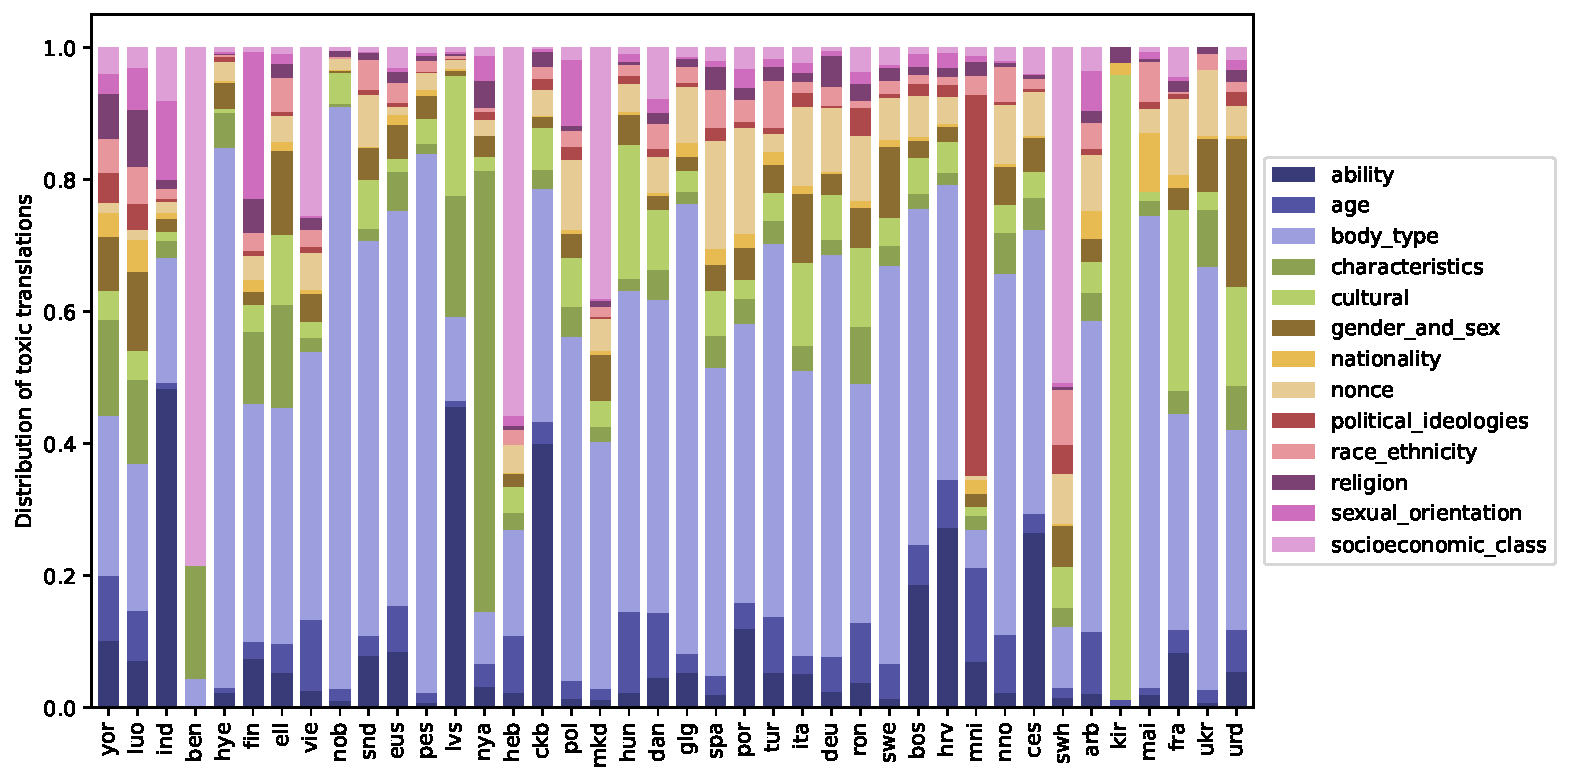
\includegraphics[width=.70\linewidth]{figures/rai/demographic_axis_hb_s2tt.pdf}
    \caption{\label{entoxx-toxicity-hb-s2t} (left) Added toxicity for \engx, \st in \holisticbias. Showing top 40 languages. The plotted languages are above 500 samples of added toxicity—0.1\% of the dataset. (right) Different languages differ in distributions of toxic terms as a function of demographic axes, with some languages’ toxicity being dominated by only one or two axes.  The figure shows the number of outputs with added toxicity per language both for \mfourtlg (orange) and \whisperlarge + \nllbmedium cascaded systems (blue).
}
\end{figure}


\paragraph{Automatic Toxicity Detection on \holisticbias Dataset}  %
\Cref{entoxx-toxicity-hb-s2t} (left) shows results for \st languages with the highest added toxicity when translating \holisticbias from \engx (note that \holisticbias is only available in English).%
Here, we observe a slightly higher amount of added toxicity compared to \fleurs for \st and a slightly lower amount for \sst. Overall, \holisticbias shows a prevalence of added toxicity of 0.19\% for \st and 0.13\% for \sst, averaged across languages. 
For \st, there are 84 languages that are affected by added toxicity. When looking at added toxicity per sentence, less than 0.003 \% of the outputs contain more than one added toxicity token. 
Figure \ref{entoxx-toxicity-hb-s2s} (left) shows results for \sst languages when translating the \holisticbias dataset. %
In total, there are 34 languages with added toxicity. %

For \st, the \whisperlarge + \nllbmedium cascaded combination adds toxicity by 29\% averaged in languages and added toxicity is prevalent in 81 languages. \mfourtlg reduces the amount of added toxicity by 34\%.

Through manual inspection, when comparing toxic words detected in \st translation but not in \sst, we observed that the word occurrences are similar with minor differences. We hypothesize that using ASR before toxicity detection tends to cause false negatives, which would explain the high decrease in added toxicity from \st to \sst (from 0.19\% to 0.13\%), which also happened in \fleurs\ (from 0.21\% to 0.16\%). For example, in the case of English to Catalan, the word "merda" in the \sst output is usually written as "mereda", and therefore not identified by ETOX. This type of example brings light to the limitations presented by detection based on tokens in a blacklist. %

Following previous work \citep{costajussa2023toxicity}, we perform an analysis of toxicity per \holisticbias' axes and report them in Figures \ref{entoxx-toxicity-hb-s2t} and \ref{entoxx-toxicity-hb-s2s} (right). Figures show the distribution of toxic translations per category and how they vary per language. We see that different languages differ in their distributions of toxic terms as a function of demographic axes. For most languages, the toxicity distribution across an axis is proportional to the axis' overall share. For instance, the main category in terms of volume is 'body type', representing 25\% of the dataset. This same category tends to accumulate a larger amount of toxicity as well. However, for some languages the toxic sentences appear to be highly concentrated in a particular axis—such is the case for Bengali (80\% socio-economic status), Nyanja (66\% characteristics), and Kyrgyz (94\% cultural) to name a few.

The categories that have a higher concentration of toxicity for \st and \sst are nonce (0.79\% and 0.46\%) and sexual orientation (0.62\% and 0.35\%). Nonce category (nonsense) is a bit of an outlier as far as terms are concerned because they do not specifically refer to any demographic groups. In terms of categories for least added toxicity, those would be age for \st (0.37\%), and political ideologies for \sst. 

\begin{figure}[h!]
    \centering
\noindent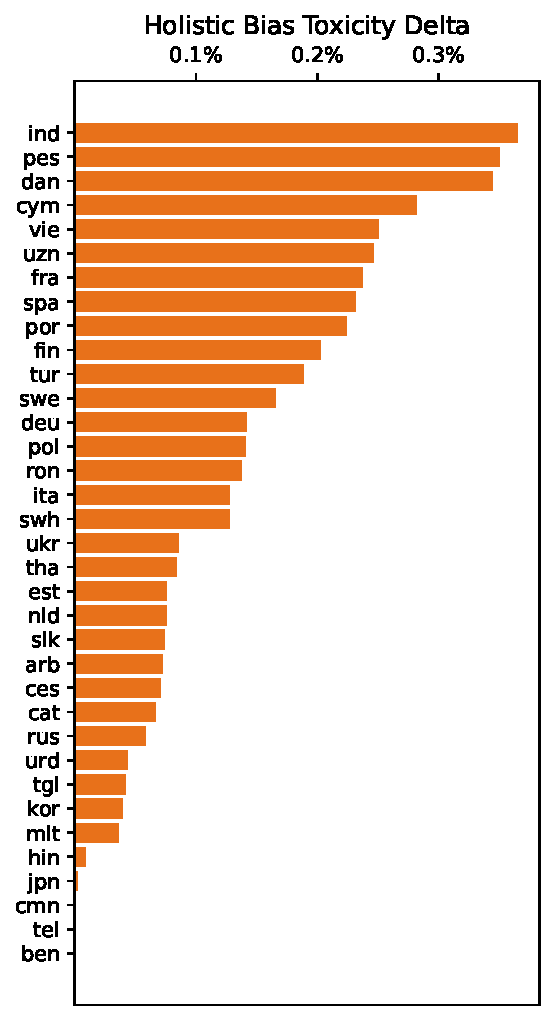
\includegraphics[width=.28\linewidth]{figures/rai/butterfly_hb_s2st.pdf}
\noindent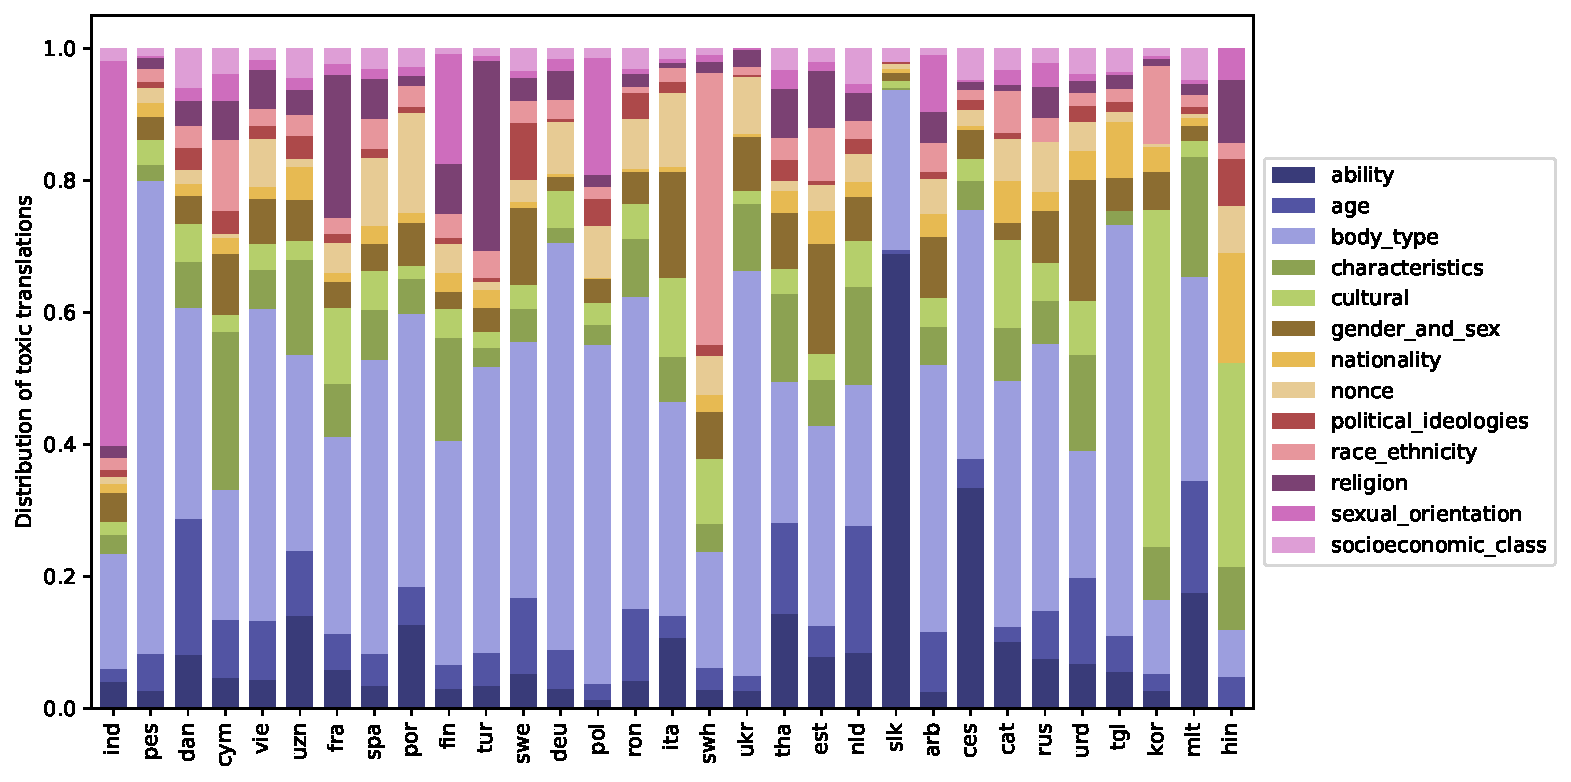
\includegraphics[width=.70\linewidth]{figures/rai/demographic_axis_hb_s2st.pdf}
    \caption{\label{entoxx-toxicity-hb-s2s} (left) Added toxicity for \engx, \sst in \holisticbias. Showing all target languages. (right) Similarly to \st, different languages differ in distributions of toxic terms as a function of the demographic axis, with some languages’ toxicity being dominated by only one or two axes. 
}
\end{figure}

























    

\paragraph{Human evaluation of added toxicity detection} 

As explained in Section \ref{sec:appendix:rai:rai_limitations}, word-list-based toxicity detection techniques are known to produce a substantial number of false positives.
These are typically due to one of two main factors: tokenization issues and toxicity list items that are only toxic in certain contexts.

We perform a human error analysis of all detected items, and determine whether these are true positives (TP) or false positives (FP) on the following translation outputs:
\begin{itemize}
    \item \fleurs outputs in the \st modality and both sets of translation directions (\engx and \xeng), and for both \mfourt and baseline systems (\mfourtlg, \whisperlarge, \whisperlarge + \nllbmedium, \whisperlarge + \yourtts), %
    \item \holisticbias outputs in the \st and \sst modalities and only the \engx set of directions for the \mfourtlg system.
\end{itemize}



\textit{Different results on \holisticbias and \fleurs} The main difference between \holisticbias and \fleurs, comparing only the comparable set of directions (i.e. \engx) is that the TP and FP rates follow opposite trends:
97–98\% of detected items are TP in \holisticbias, whereas 81–84\% of detected items are FP in \fleurs.

\textit{Comparison between the \sst and \st modalities on \holisticbias}. The S2TT modality produced more (1.2 x) detected added toxicity than S2ST.
The percentages of TP and FP are roughly the same in both modalities, and follow the same clear trend (between 97 and 98\% of detected items are TP).

\textit{Comparison between M4T and baseline on FLEURS in the S2TT modality}.
In the eng-x directions both systems show similar results: 
The baseline system produces more detected added toxicity (~1.2x) than M4T;
Between 80–84\% of detected items are FP for both systems.
In the x-eng directions more differences can be observed:
The baseline system produces 2x the number of detected added toxicity produced by M4T;
While in the baseline system the reversal in direction polarities is mirrored by a reversal in the TP-to-FP ratio (eng-x: 18.6\%TP, 81.4\% FP; x-eng: 80.3\% TP, 19.7\% FP), this does not occur in the M4T system (eng-x: 16.3\%TP, 83.7\% FP; x-eng: 42.3\% TP, 57.7\% FP).

These results re-confirm the real toxicity mitigation found with automatic metrics.

\paragraph{Ethics statement} All annotators who worked on the human evaluation of detected toxicity are team members who are aware of the toxic nature of the samples prior to analyzing them.

\subsubsection{Toxicity key findings and contributions}

To summarize, our key findings and contributions include: (1) proposing a metric for speech toxicity detection for languages at scale (\asretox), (2) showing that while levels and types of added toxicity vary significantly as a function of language and dataset, added toxicity in our systems has a relatively low prevalence (varying from 0.11\% to 0.21\% across modalities, language directions, and datasets), and %
(3) our evaluation against the state-of-the-art shows that \mfourtlg reduces toxicity by 51\% across modalities and language directions in \fleurs and by 34\% in \holisticbias for \engx in \st{}. {\color{red}A manual analysis of toxicity detection outputs confirm this toxicity mitigation rate holds on real toxicity.} %
    


\subsection{Bias}
\label{apx:holisticbias}


\subsubsection{Motivation}

Unequal training datasets can lead to demographic and representational biases that affect our models and their generated outputs. These biases can adversely impact users by perpetuating allocation biases when used in situated contexts. In recent years, the MT field has made significant progress in uncovering \citep{prates:2020}, evaluating \citep{stanovsky-etal-2019-evaluating,renduchintala-etal-2021-gender, costa-jussa-etal-2022-evaluating,bentivogli-etal-2020-gender}, or even mitigating many of these forms of biases \citep{renduchintala-williams-2022-investigating}. However, much work lies ahead of us when it comes to this domain of research. 










\textbf{Related work}  \multilingualholisticbias dataset \citep{costa2023multilingual} consists of an extension to \holisticbias. It contains translations for three different patterns and 118 descriptors, available in 50 different languages. Depending on whether gender inflection exists in a language, each language has one or two references. Each translated sentence includes the masculine, neutral and, when applicable, a feminine iteration.
The dataset enables quantification of gender biases across demographic aspects for \mt and has the highest language coverage at the time of writing. Previous work on this matter is mostly in text \citep{stanovsky-etal-2019-evaluating,renduchintala-etal-2021-gender,levy-etal-2021-collecting-large,costajussaetal:2022,renduchintala-williams-2022-investigating} and tend to be English-centric, with few demographic axes and multilingual references. Similar efforts for the speech modality remain sparse \citep{costa-jussa-etal-2022-evaluating, bentivogli-etal-2020-gender}.

\textbf{Contributions.} In this work, we used \multilingualholisticbias and its speech extension (described in the following section) to compare the performance of \st\ and \sst. The \engx direction allows comparing performance in the presence of masculine or feminine references, and the \xeng direction enables robustness comparisons in translations when we alter gender inflection. A typical example of the language pair of English-Spanish would be "I'm a homemaker" and the corresponding translations "Soy amo de casa" and "Soy ama de casa" in Spanish. When translating from English to Spanish, we can measure if the system overgeneralizes to one gender, while in the other direction, we can evaluate the robustness of the translation to gender inflection.

\subsubsection{Bias Experimental Framework}
\label{subsec:biasexperimental}

 

\paragraph{Dataset: Speech Extension of \multilingualholisticbias} 
In order to compare the performances across modalities (\sst and \st), we begin by extending the \multilingualholisticbias dataset from text to speech by using the TTS model\footnote{https://github.com/facebookresearch/fairseq/tree/main/examples/mms\#tts-1} provided by \cite{mms}. Due to the limitations of this TTS model in correctly generating speech for numbers, we manually converted all numerical numbers to words for each language. For instance, the sentence “I have friends who are 50 years old.” is transformed into “I have friends who are fifty years old.” After processing through TTS, we obtained the synthesized speech for 325 sentences across 19 languages. These languages are supported both by MMS-TTS and the \multilingualholisticbias\footnote{Arabic, Belarusian, Bulgarian, Catalan, Czech, Danish, German, Greek, French, Italian, Lithuanian, Latvian, Marathi, Dutch, Portuguese, Romanian, Russian, Slovak, Slovenian, Spanish, Swedish, Tamil, Thai, Ukrainian, Urdu.} dataset  \citep{costa2023multilingual}. For each of these languages (except English), we generated two speeches, one for each set of gendered texts.

\paragraph{Language directions and modalities}
We use this generated TTS data as input for \st\ and \sst and as a reference for \sst. We conducted the translations in two directions—\engx and \xeng. Concretely, in \xeng, we translated both masculine and feminine versions of the speech. 
It's worth noting that some target languages are not available in the \mfourt\ \sst model, so we performed translations on only 17 languages for the \sst~ task in the \engx direction. For \st in \engx, we have all languages included in the \multilingualholisticbias dataset (n=25). For reference, the complete language list used in our experiments can be found in Table \ref{tbl:rai-bias-language-summary}.
\begin{table}[ht]
    \begin{center}
    \small
   \begin{tabular}{lm{6cm}m{6cm}}
   \toprule
    & \hfil$\textbf{\xeng}$ & \hfil$\textbf{\engx}$ \\
    \midrule
    \textbf{\sst} & \multirow{2}{*}{\makecell[l]{\\arb,bul,cat,deu,ell,fra,lvs,mar,nld,\\por,ron,rus,spa,swe,tam,tha,ukr,urd}} & arb,cat,ces,dan,deu,fra,ita,nld,por,ron, rus,slk,spa,swe,tha,ukr,urd \\ \cline{1-1}\cline{3-3}
    \textbf{\st} & 
    & arb,bel,bul,cat,ces,dan,deu,ell,fra,ita, lit,lvs,mar,nld,por,ron,rus,slk,slv,spa, swe,tam,tha,ukr,urd \\
    \bottomrule
    \end{tabular}
    \end{center}
    \caption{List of language codes in the bias evaluation experiments, organized by task and language direction.}
    \label{tbl:rai-bias-language-summary}
\end{table}


\paragraph{Evaluation} %
In terms of evaluation metrics for \st,
we used chrF as reported in Table \ref{tbl:eval:metrics}, except that nw:2 was changed to nw:0. 
Instead of using \bleu as the quality metric, we used chrF because it is more equipped to handle shorter utterances, which better suits the evaluation of the
\multilingualholisticbias dataset. This dataset is relatively small (325 utterances) and with short sentences (on average, 6 words per utterance) \citep{costa2023multilingual}. 
In this context, we find chrF more adequate for comparison \citep{ma-etal-2019-results}, since \bleu quickly drops when not enough lengthy n-grams are matched. For \sst, we used \asrchrf.\footnote{The transcription is done by \whisperlarge and \whispermedium \citep{whisper} for \engx and \xeng respectively. chrF has been calculated the same way as \st except that in \sst the text from both prediction and reference are normalized.} 
and \blaser proposed in this work. It is worth noting that when evaluating \blaser, we included only 14 languages (including English)\footnote{The list of 
language codes for these 14 languages: arb,cat,deu,eng,fra,nld,por,ron,rus,spa,swe,tha,ukr,urd.} for the \engx direction (overlaps between the languages from the generated TTS data and the languages available in our \sst model). %
Additionally, since MMS-TTS generations are not deterministic, we repeated the measurements three times for both \sst and \st. The final metric values are then averaged to ensure robustness and accuracy in our evaluations.

\paragraph{Models} We used the \mfourtlg model and several different baselines. For \xeng\ \st, we employed \whisperlarge~\citep{whisper}. As for \xeng\ \sst, we used  \yourtts ~\citep{casanova2022yourtts} to generate synthesized speech from the output of \whisperlarge\ \st. For \engx\ \st, we utilized a cascaded system: \asr from Whisper Large-v2~\citep{whisper}, followed by \mt via \nllbmedium \citep{nllb2022}.
For \mfourtlg\ \st, we used a beam size of ten. For \mfourtlg\  \sst, we set the beam size to five for both the first pass decoder and the second pass decoder. As for the baseline, we set the beam size to five for \nllbmedium and used the default values for \whisperlarge and \yourtts.

\subsubsection{Bias evaluation results}

This section focuses on analyzing gendered translations when using neutral inputs (\engx) and the gap in translation performance between inputs that only differ in gender (\xeng). 

\begin{figure}[h!]
\centering
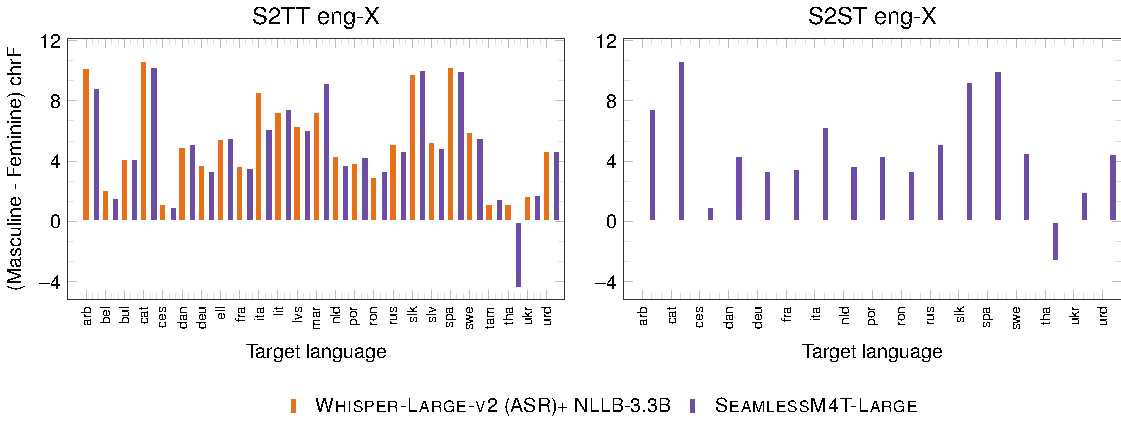
\includegraphics[width=\linewidth]{figures/rai/bias/bias_gender_engx.pdf}
\caption{Left: The chrF points difference between masculine and feminine forms for \engx\ \st using English speech as source and X text translation (masculine or feminine) as reference. Right: The \asrchrf points difference between masculine and feminine forms for \engx\ \sst using English speech as source and X text translation (masculine or feminine) as reference.}
\label{fig:mhb_en-xx_s2t_s2s}
\end{figure}

\begin{figure}[h!]
\centering
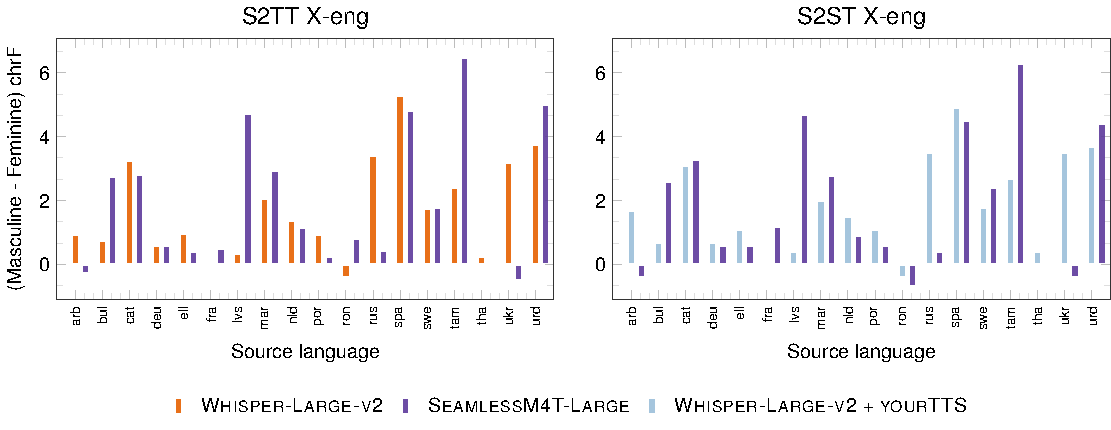
\includegraphics[width=\linewidth]{figures/rai/bias/bias_gender_xeng.pdf}
\caption{(left) The chrF points difference between masculine and feminine for \xeng\ \st using X speech synthesized by the masculine or feminine version of the text and English text as a reference. (right) The \asrchrf points difference between masculine and feminine forms for \xeng\ \sst using X speech synthesized by the masculine or feminine version of text and English text as reference.}
\label{fig:mhb_m4t_vs_baseline}
\end{figure}

\begin{figure}[h!]
\centering
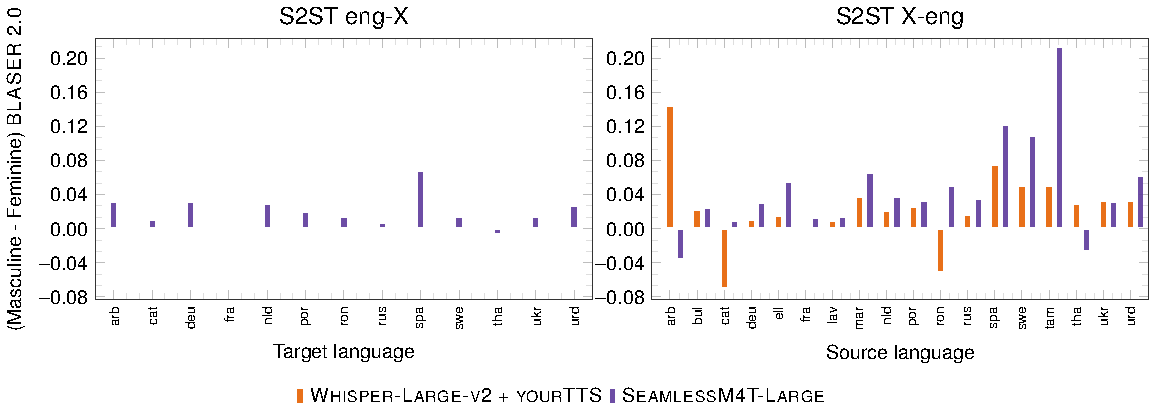
\includegraphics[width=\linewidth]{figures/rai/bias/bias_gender_blaser.pdf}
\caption{(left) The supervised \blaser points difference between masculine and feminine forms for \engx\ \sst using English speech as the source and X text translation (masculine and feminine) as reference. The results are averaged from three experiments. (right) The supervised \blaser points difference for \xeng\ \sst using X speech synthesized by the masculine or feminine version of text and English text as reference.}
\label{fig:mhb_m4t_vs_baseline_blaserv2}
\end{figure}




\begin{table}[ht]
\centering
\small
\begin{tabular}{@{}lccccc@{}}
\toprule
&\multicolumn{5}{c}{\bf \st}\\\cmidrule{2-6}
{\bf Axis} & Masculine & Feminine & Average & Count & Diff\\
\midrule
Cultural & 11.4 & 9.5 & 10.4 & 350 & 1.9 \\
Body type & 14.2 & 12.9 & 13.6 & 3750 & 1.2 \\
Socioeconomic class & 14.6 & 13.3 & 13.9 & 400 & 1.3 \\
Religion & 15.5 & 13.7 & 14.6 & 1800 & 1.8 \\
Gender and sex & 16.0 & 15.1 & 15.5 & 1800 & 1.0 \\
Ability & 16.6 & 15.2 & 15.9 & 3300 & 1.3 \\
Race ethnicity & 17.4 & 15.7 & 16.5 & 900 & 1.7 \\
Characteristics & 18.2 & 16.2 & 17.2 & 1900 & 2.0 \\
Nationality & 18.1 & 16.7 & 17.4 & 300 & 1.4 \\
Sexual orientation & 18.5 & 16.7 & 17.6 & 700 & 1.8 \\
Age & 18.6 & 16.6 & 17.6 & 900 & 1.9 \\
\midrule
&\multicolumn{5}{c}{\bf \sst}\\\cmidrule{2-6}
{\bf Axis} & Masculine & Feminine & Average & Count & Diff\\

\midrule
Cultural & 12.2 & 10.3 & 11.3 & 238 & 1.9 \\
Body type & 14.2 & 13.0 & 13.6 & 2550 & 1.2 \\
Socioeconomic class & 14.4 & 13.1 & 13.7 & 272 & 1.3 \\
Religion & 16.3 & 14.5 & 15.4 & 1224 & 1.9 \\
Gender and sex & 16.7 & 15.7 & 16.2 & 1224 & 1.0 \\
Ability & 16.9 & 15.5 & 16.2 & 2244 & 1.4 \\
Age & 17.7 & 15.8 & 16.7 & 612 & 1.9 \\
Characteristics & 17.7 & 15.9 & 16.8 & 1292 & 1.8 \\
Race ethnicity & 18.0 & 16.4 & 17.2 & 612 & 1.7 \\
Sexual orientation & 18.4 & 16.9 & 17.7 & 476 & 1.5 \\
Nationality & 18.7 & 17.3 & 18.0 & 204 & 1.3 \\
\bottomrule
\end{tabular}
\caption{ Results on mean per axis (across descriptor, template, and language): chrF on \st (top) and \asrchrf on \sst (bottom) results. Columns (from left to right): masculine references, feminine references, average between the two, the total number of measurements (Count), and the difference between masculine and feminine (Diff). The rows are sorted in ascending order by the average chrF for \sst and \st, respectively. The axes are defined in \holisticbias—for more details, refer to Table 5 in the original paper \citep{smith-etal-2022-im}.}\label{tbl:m4t-en-xx-demographic}
\end{table}

\paragraph{\engx.} In our analysis, we utilize the masculine or the feminine human translations of the non-English language as references. The source for this analysis is the English (eng) \multilingualholisticbias dataset, comprising a collection of unique sentences with ambiguous gender. %
Figure \ref{fig:mhb_en-xx_s2t_s2s} shows the results per target language, evincing the following patterns:

\begin{itemize}
    \item In \mfourtlg \st, the translation quality deteriorates for all the languages except Thai when using the feminine reference, and is especially noticeable in languages like Catalan (with a significant 10.3 chrF points difference), Slovak (10.1), and Spanish (10.0). For the \whisperlarge + \nllbmedium combination, a decline in translation quality is observed across all languages. The highest differences are found in Catalan (10.7), Spanish (10.3), and Arabic (10.2). It's worth mentioning that the biases' distribution over languages is similar between \mfourtlg and the \whisperlarge + \nllbmedium combination, with Thai being the only exception. 
\item In \sst, we noticed similar trends in relation to \st, where translation quality is lowered in all languages (except Thai) when assessing with the feminine reference. The highest differences are with Catalan (10.7 \asrchrf points difference), Spanish (10.0), and Slovak (9.3). %

\end{itemize}


The left panel of Figure \ref{fig:mhb_m4t_vs_baseline_blaserv2} shows the results for automatic speech evaluation by way of \blaser. We observe similar trends in the \asrchrf metric. The translation quality deteriorates by an average of 0.02 supervised \blaser points across languages when evaluating with the feminine reference for all languages except Thai. Interestingly, the evaluation for French reveals a negligible difference. The highest differences are found in Spanish (0.07), followed by German (0.03).

These differences show that when no gender information is available in the source sentence, the model will prefer to translate to the masculine form in the target language. Note that for some languages (like Spanish or French), the plural masculine form is indistinguishable from the plural generic form.

\paragraph{\xeng.} Our main objective is to assess the translation quality when starting from a gendered sentence and translating it into English. %
As such, we aim to measure the model's robustness with regard to gender bias and its ability to handle translations between languages that mark grammatical gender towards English. Figure \ref{fig:mhb_m4t_vs_baseline} shows the results per source language for \mfourtlg and \whisperlarge or \whisperlarge + \yourtts. We observe that:

\begin{itemize}
    \item In \st, the performance is better when translating from the masculine reference for most languages (15 out of 18 for \mfourtlg and 16 out of 18 for the \whisperlarge). However, they have different biases towards different languages. The highest differences between the masculine and feminine forms in \mfourtlg are with Tamil (6.4 chrF points difference) and Urdu (5.0).\footnote{We find that in our experiment, Arabic shows the bias toward the cases when translated from feminine version, which contrasts with the findings in the \multilingualholisticbias \citep{costa2023multilingual} where Arabic exhibited significantly higher performance when translating from the masculine version. We hypothesize that this difference is attributed to our use of a different language code "ara" instead of "arb" when applying the MMS-TTS.} On the other hand, the highest differences in \whisperlarge are with Spanish (5.3), Urdu (3.8), and Russian (3.4).

\item In \sst, we observe similar outcomes to those in \st. The model quality is mostly better when translating from masculine cases, as evident in 14 out of 18 languages for \mfourtlg and 17 out of 18 for the \whisperlarge + \yourtts combination. The most significant differences between masculine and feminine sources in \mfourtlg are found in Tamil (with an \asrchrf point difference of 6.3) and Spanish (4.5). The highest differences in \whisperlarge are in Spanish (4.9), Urdu (3.7), and Ukrainian (3.5). %

\end{itemize}

The right panel of Figure \ref{fig:mhb_m4t_vs_baseline_blaserv2} demonstrates the performance comparison using \blaser. Like the findings in \asrchrf, the translation quality generally improves when translating from masculine cases, which is observed in 16 out of 18 languages and 15 out of 18 languages for \mfourtlg and \whisperlarge + \yourtts\ respectively. The highest differences for \mfourtlg are with Tamil (0.21 supervised \blaser points), Spanish (0.12), and Swedish (0.11). For \whisperlarge + \yourtts, the highest differences are found in Arabic (0.14), Spanish (0.075), and Tamil (0.05).

\paragraph{Average comparison across directions and modalities} Table \ref{tbl:m4t_baseline_xx_en_average} presents the average scores per gender and the comparison with the corresponding baseline.\footnote{For \engx\ \sst, we report only the performance for the \mfourtlg in absence of baseline.} $\Delta$ corresponds to the relative variation between genders computed as follows:
\begin{equation*}
\Delta = \omega(M-F)/\omega(min(M,F)), \omega \in \{ \textsc{chrF}, \asrchrf, \blaser \}
\end{equation*}
As mentioned, in \engx, we evaluated translations from neutral to gendered forms and observed the overgeneralization towards one gender, whereas in \xeng, we evaluated the robustness of translating content that only differs in their gender inflection. Focusing sorely on the results of \mfourtlg, we noticed that, except for the evaluation outcomes in \blaser, the difference in performance between the masculine and feminine forms is more pronounced for overgeneralization than for robustness. Turning our attention to the performance comparison, we find that when it comes to overgeneralization, \mfourtlg slightly outperforms \whisperlarge + \nllbmedium. As for the outcome related to the robustness, \mfourtlg falls short against \whisperlarge in \st but outperforms \whisperlarge + \yourtts in \sst. We further noticed a higher percentage gap in \asrchrf than for \blaser. This may imply that ASR (from \asrchrf) adds some extra biases.




\begin{table}[ht]
\centering
\small
\begin{tabular}{ccccc}
\toprule
&&\multicolumn{3}{c}{\textbf{\engx \mfourt/\whisperlarge + \nllbmedium}}\\\cmidrule{3-5}
& & Feminine Reference & Masculine Reference & $\Delta$ \%\\
\midrule
{\st}& chrF & 45.0/\textbf{47.4} & 49.9/\textbf{52.7} & \textbf{10.9}/11.2\\
\midrule
\multirow{2}{*}{\sst} & \asrchrf & 44.9 & 49.7 & 10.6\\
& \blaser & 3.6 & 3.7 & 0.6\\
\midrule
&& \multicolumn{3}{c}{\textbf{\xeng\ \mfourt/\whisperlarge (+ \yourtts)}}\\\cmidrule{3-5}
& & Feminine Source & Masculine Source & $\Delta$ \%\\
\midrule
{\st} & chrF & \textbf{52.4}/50.4 & \textbf{54.3}/52.1 & 3.7/\textbf{3.4}\\
\midrule
\multirow{2}{*}{\sst} & \asrchrf & \textbf{53.1}/52.2 & \textbf{55.0}/54.0 & \textbf{3.5}/\textbf{3.5}\\
& \blaser & \textbf{3.5}/2.7 & \textbf{3.6}/2.8 & 
\textbf{2.9}/3.7\\
\bottomrule
\end{tabular}
\caption{The averaged points across modalities and genders for assessing the overgeneralization (\engx) and the robustness (\xeng). ${\Delta}$ represents the relative difference between masculine and feminine (${\Delta = \omega(M-F)/\omega(min(M,F)), \omega \in \{ chrF, \asrchrf, \blaser \}}$).}
\label{tbl:m4t_baseline_xx_en_average}
\end{table}

\paragraph{Demographic analysis}
We conducted a similar analysis to that in \cite{costa2023multilingual}. Table \ref{tbl:m4t-en-xx-demographic} shows the mean chrF or \asrchrf at the sentence level on the \multilingualholisticbias axes translations, averaged across descriptors, templates, languages, and masculine vs. feminine references. Among all the axes, we find that cultural, body type, socioeconomic class, and religion are most sensitive to quality disruptions. Furthermore, when considering the difference between masculine and feminine references and the number of effective samples, we observe that both \sst and \st show the highest bias in the ability, body type, religion, and characteristics axes. These observations align with the findings reported in \cite{costa2023multilingual} pertaining to \mt.

\subsubsection{Gender data representation}



Based on our concurrent work \citep{muller-etal-2023-pipeline}, we discuss the representation bias of several datasets by focusing on how different genders are represented using lexical matching. %
The closest work that studies gender representation in data is \cite{choubey-etal-2021-gfst}, where the authors took on this research question using a synthetic dataset. The authors, however, did not share the details of the lexical nouns used to extract this representation. 

\holisticbias \citep{smith-etal-2022-im} provides a list of gendered nouns and pronouns. We rely on this list to track how many sentences in our data sets contain gendered markers.
Since our analysis is only in English, we tokenize for word boundaries using python word-boundary regular expression ($\backslash$b). As lexical terms, we limited the vocabulary to make our approach scalable to multiple languages \citep{muller-etal-2023-pipeline}. This vocabulary includes 11 masculine nouns\footnote{man, men, bro, bros, guy, guys, boy, boys, father, fathers, dad, dads, son, sons, husband, husbands, grandfather, grandfathers, grandpa, grandpas, brother, brothers.}; 4 masculine pronouns,\footnote{he, him, his, himself.}; 10 feminine nouns\footnote{woman, women, lady, ladies, girl, girls, mother, mothers, mom, moms, daughter, daughters, wife, wives, grandmother, grandmothers, grandma, grandmas, sister, sisters}, and 4 feminine pronouns\footnote{she, her, hers, herself.}. We matched single words, hence we report the number of words out of the total number of words in the dataset. %
 Figure \ref{fig:datarepr} summarizes the results of the gender representations for several English evaluation and training datasets. Results show that masculine representation is predominant in most of the datasets. Extremely low representations of gender (i.e., low matching of gendered words based on our selected vocabulary) are found in EuroParl, \fleurs, and \flores datasets. However, this low representation is the trade-off to make our approach scalable to multiple languages. This scalable effort on data characterization could potentially be used for the purpose of balancing datasets to mitigate gender biases.


\begin{figure}[ht!]
\centering
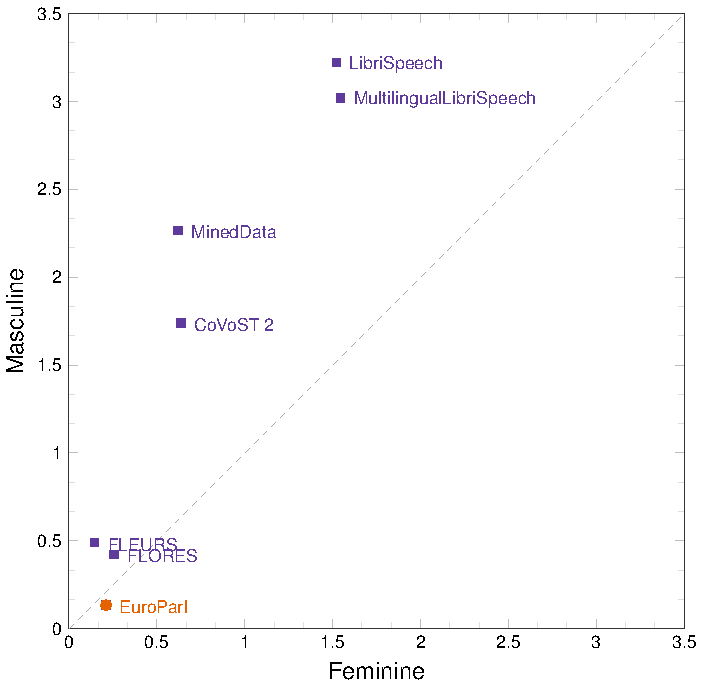
\includegraphics[width=0.8\linewidth]{figures/evaluation/bias_datasets.pdf}
\caption{Gender representation of English evaluation datasets (EuroParl, \flores, \fleurs, \covost, LibriSpeech and MultilingualLibriSpeech), and training mined data (\mineddata). Vertical axis show the percentage of masculine representation and horizontal axis show the percentage of feminine representation.}\label{fig:datarepr}
\end{figure}




\subsubsection{Bias Key Findings}

In this section, we conducted a set of comprehensive evaluations on translation biases for \st\ and \sst. We demonstrate the following: (1) in the absence of gender information, \mfourtlg exhibits an average preference of $\sim$10\% towards translating to the masculine form (for both modalities); (2) utilizing feminine form as the source input leads to lower quality English translations compared to its masculine counterpart, showing a lack of robustness against gender inflection by $\sim$3\% ; (3) \mfourtlg gets comparable bias results to the state-of-the-art, %
 and (4) our gender representation analysis reveals an overrepresentation of masculine lexica compared to feminine in the analyzed datasets.
More importantly, these findings pave the way towards standardizing the bias evaluation of speech translation at a massive scale.



\subsection{Limitations}\label{sec:appendix:rai:rai_limitations}
Due to the lack of available model-based techniques that could be applied to added toxicity or gender imbalance detection in this multimodal and massively multilingual setting, we used string-matching techniques that present known limitations.

First, the use of toxicity lists with ETOX for added toxicity detection shares the same limitations with other word list-based detection techniques, which were previously discussed at length in \cite{nllb2022} and \cite{costajussa2023toxicity}. Briefly, the two main limitations of word list-based detectors are (1) their tendency to over-detect terms that are only toxic in specific contexts, and (2) their reliance on precise tokenization, which is more difficult to achieve in non-segmenting or highly agglutinative languages. When dealing with speech outputs, the process of using ASR before lexical matching adds one more source of error, which tends to lead to false negatives. This particularly affects the directions of \engx, since ASR tends to be of lower quality for non-English languages.

Second, the use of noun lists for the detection of linguistic gender imbalance in large datasets shares all of the limitations of word list-based techniques previously stated, along with the added difficulty of relying on linguistic gender clues as a proxy for overall gender representation. Indeed, linguistic gender assignment does not follow the same pattern across all languages that mark gender, especially when it comes to inclusive plural forms (i.e., plural forms referring to groups that include more than one gender). In addition to general limitations, the use of a specific and limited set of 30 nouns (selected to mirror those used to build the \holisticbias dataset) does not guarantee that results can be generalized to all other sets of nouns that could be used to investigate gender representation (e.g., occupation nouns).





